\chapter{对 ZUC 算法的分析方案}
\label{chap:attack}

\section{差分功耗分析的一般步骤}
\label{sec:dpa}
功耗分析通常包含简单功耗分析(Simple Power Analysis)和差分功耗分析(Differential Power Analysis)。

简单功耗分析通常只需要少量的功耗曲线,就能揭示密码设备中的有用信息。简单功耗分析通常适用于功耗曲线特征较为明显的密码设备,比如出现明显的波峰和波谷,以及呈现出多个周期性的重复段落。如果攻击者对密码设备中运行的程序有一定的预备知识,那么就能推测出功耗曲线的不同段落在执行何种操作,就有可能进一步掌握设备的更多信息。

差分功耗分析则需要大量的功耗迹。大量功耗数据带来的好处就是更强大的分析和攻击能力,也不需要对设备的构造和执行的程序有详细的了解,一般情况下,只要掌握设备运行的算法流程就足够实施分析和攻击了。

因此,我们的关注重点就放在差分功耗分析上。

\vspace*{0.5\baselineskip}

下面我们来介绍一下差分功耗分析的一般流程:\cite{paa_cn}

\begin{enumerate}
\item \textbf{选取合适的算法中间值位置:}一个好的中间值,应该尽可能地区错误的猜测和正确的猜测。因此,在密码算法中,通常选择非线性函数的输出作为差分功耗分析的中间值。由于在运行算法和采集功耗时,攻击者往往只能获得明文或者密文,因此通常只能对算法的第一轮加密或者最后一轮加密进行攻击。因此,选取的中间值最好能够出现在第一轮或者的最后一轮。选取不同的中间值,会对攻击效果产生很大的影响,因此需要根据不同的算法和具体的实验条件,选取最合适的算法中间值。
\item \textbf{采集设备运行时的实际功耗曲线:}这一部分没有什么技术难度,不过值得一提的是,如果合理地选择功耗曲线采集和结束的位置,就能得到对齐较好的曲线,方便后续的分析和处理。采集环境也要尽可能地排除外界因素的干扰,以提高功耗曲线同数据和操作的相关性,增大信号的信噪比。更多具体的细节已经在上一小节阐述了。
\item \textbf{根据算法计算理论中间值:}对某个具体的密码算法而言,密钥通常是最重要也是最机密的信息,攻击者唯一无法知晓的也是这一部分。对全部位数的密钥进行穷举猜测是不可能做到的,因此攻击者常常需要在选择合适的中间值的前提下,尽可能地降低中间值和全部密钥之间的相关性。或者说,攻击者应该尽可能选取只依赖少部分密钥的中间值,这样就能大大减少猜测的可能情况,提高攻击的效率。由于密码算法通常是公开透明的,因此已知明文和猜测密钥的情况下,是可以计算出适合的理论中间值的。
\item \textbf{使用合适的功耗模型将理论中间值转换为假设功耗值:}算法的中间值通常是某个字节或者比特,和算法有关。由于中间值的值域很大,因此对所有可能的中间值建立一个具体的模型是不现实的。所以有必要采用合适的功耗模型,缩小猜测空间,将中间值转换成假设功耗值。常用的功耗模型包括汉明重量模型、汉明距离模型以及零值模型。功耗模型之间各有利弊,需要根据实际的实验情况和攻击效果选取最合适的模型。
\item \textbf{分析假设功耗值和实际功耗曲线,挖掘所需的信息:}这部分通常涉及到一定的统计学知识,需要攻击者具备较好的数学基础。在分析曲线的特征之前,通常还要对功耗曲线进行预处理,比如对齐和滤波,减少噪声,提高信噪比,从而能够更好地利用功耗曲线中的有效信息。此外,高效地处理大量的数据也是一个需要仔细考量的问题,差分功耗分析往往会采集成千上万甚至是百万条曲线,如何编写性能优异的算法,或者是并行化处理,都会很大程度上影响分析的速度和效果。除了常用的相关系数攻击之外,模板攻击也很有效。攻击者应该尽可能地设计好的算法,从而减少所需的功耗曲线条数,这样就能大大减少攻击的时间和成本。
\end{enumerate}

\vspace*{0.5\baselineskip}

图 \ref{fig:dpa} 展示了差分功耗分析攻击的第 3 -- 5 步。

\begin{figure}[htbp]

    \centering
    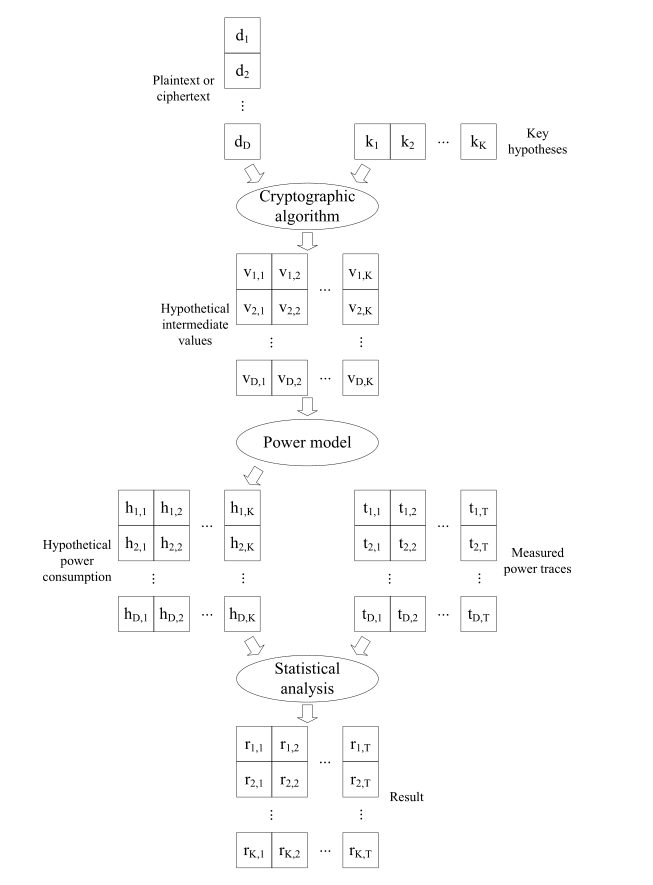
\includegraphics[height=.6\textheight]{../images/dpa.png}
    \caption{差分功耗分析的典型流程\cite{paa_en}}
    \label{fig:dpa}
\end{figure}

\section{对 ZUC 算法实施差分功耗分析攻击}

在 ZUC 算法中,唯一未知的信息就是初始密钥,其他的常量和明文都是已知的。因此我们的攻击目的就是得到密钥的信息。

差分功耗攻击最核心的思想是,假设功耗值和实际功耗值之间是有关联的。而要想假设功耗值尽可能贴合实际功耗值,就需要选择合适的中间值,采用合适的功耗模型。一般而言,中间值通常选择算法中非线性变换的部分,因为如果输入稍有不同,非线性变换的输出就会出现较大的差异,因此,正确的输入和错误的输入产生的差异将比线性变换更加明显,就可以有效地区分出正确的输入和错误的输入。功耗模型通常选择汉明重量模型或者比特模型,为了方便,我们这里采用汉明重量模型。

\vspace*{0.5\baselineskip}

差分功耗分析的第一步是要在硬件上实现 ZUC 算法电路,然后采集其运行时的功耗。这部分和针对其他算法的差分功耗分析没有什么差别,因此不再详细说明。我们重点关注分析 ZUC 算法中的特别之处。

\vspace*{0.5\baselineskip}

图 \ref{fig:zuc_attack} 展示了 ZUC 算法中可以利用的漏洞。在 ZUC 算法初始化阶段的第一轮打乱操作中,非线性函数中左侧寄存器的输出仅和 k9 这个密钥字节相关,右侧寄存器的输出仅和 k5 这个密钥字节相关。 \cite{zuc_attack_tangming}

\begin{figure}[htbp]
    \centering
    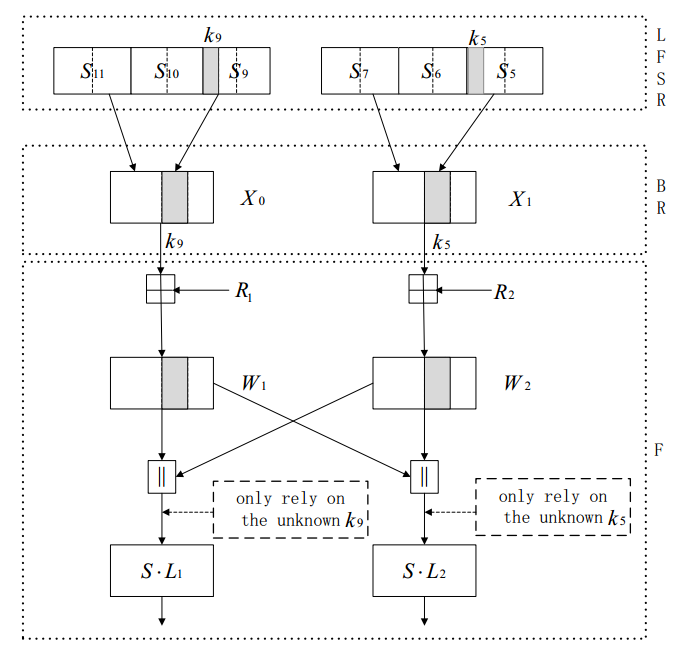
\includegraphics[height=.5\textheight]{../images/zuc_attack.png}
    \caption{非线性函数中左侧寄存器的输出仅和 k9 相关,右侧寄存器的输出仅和 k5 相关\cite{zuc_attack_tangming}}
    \label{fig:zuc_attack}

\end{figure}

因此,选择初始化阶段第一轮打乱操作中,非线性函数右半部分的输出作为我们的中间值,尝试攻击出 k5 的值。

\vspace*{\baselineskip}


% A lot to add !




选择这个位置作为中间值有两个原因:

\begin{enumerate}
    \item \textbf{这个位置仅仅和单个密钥字节(k5)相关,和其他的密钥字节没有任何关系。}这意味着我们只需要猜测 $2^8=256$ 中情况,大大减少了工作量。如果选择某个其他的中间值,很可能和多个密钥字节有关联,我们假设关联的密钥字节数为 N,那么我们就需要猜测 $2^{8 \times N}$ 中情况。可以想象,如果关联的密钥字节很多的话,我们需要猜测的可能情况就会爆炸式增长,由于我们只拥有有限的计算资源,因此这是不能接受的。
    \item \textbf{这个位置是非线性变换(S 盒置换)的输出,因而正确猜测和错误猜测之间的差异较为明显。}这一点我们在上面已经提及,因此不再赘述。
\end{enumerate}

\vspace*{\baselineskip}

选择好了中间值,我们就可以通过编程计算出所有密钥猜测(从 0 到 255,也即 16 进制的 00 到 FF)对应的的中间值。

有了中间值之后,我们就可以根据汉明重量模型,计算出理论功耗值(也就是假设功耗值)。然后我们实施相关系数攻击,也即计算假设功耗值和实际功耗值之间的相关系数(在本次实验中,这个值还需要稍微处理一下,得到更加可靠的相对相关系数),然后分析相对相关系数,值最大的即对应最优的密钥猜测。

这就是对 ZUC 算法进行功耗分析攻击的大致流程,我们将在下一小节展示相关的实验结果,并补充一些实现细节。

\section{本章小结}




我们讨论了功耗分析中简单功耗分析和差分功耗分析的异同,并且重点介绍了差分功耗攻击的基本流程和一般方法。

最后我们讨论了针对 ZUC 算法的差分功耗分析方案,除了介绍了传统的差分功耗分析的流程,还依据相关资料选取了有效的中间值,并且解释了这样选取的具体原因。